\let\negmedspace\undefined
\let\negthickspace\undefined
\documentclass[journal]{IEEEtran}
\usepackage[a5paper, margin=10mm, onecolumn]{geometry}
%\usepackage{lmodern} % Ensure lmodern is loaded for pdflatex
\usepackage{tfrupee} % Include tfrupee package

\setlength{\headheight}{1cm} % Set the height of the header box
\setlength{\headsep}{0mm}     % Set the distance between the header box and the top of the text

\usepackage{gvv-book}
\usepackage{gvv}
\usepackage{cite}
\usepackage{amsmath,amssymb,amsfonts,amsthm}
\usepackage{algorithmic}
\usepackage{graphicx}
\usepackage{textcomp}
\usepackage{xcolor}
\usepackage{txfonts}
\usepackage{listings}
\usepackage{enumitem}
\usepackage{mathtools}
\usepackage{gensymb}
\usepackage{comment}
\usepackage[breaklinks=true]{hyperref}
\usepackage{tkz-euclide} 
\usepackage{listings}
% \usepackage{gvv}                                        
\def\inputGnumericTable{}                                 
\usepackage[latin1]{inputenc}                                
\usepackage{color}                                            
\usepackage{array}                                            
\usepackage{longtable}                                       
\usepackage{calc}                                             
\usepackage{multirow}                                         
\usepackage{hhline}                                           
\usepackage{ifthen}                                           
\usepackage{lscape}
\usepackage{circuitikz}
\tikzstyle{block} = [rectangle, draw, fill=blue!20, 
    text width=4em, text centered, rounded corners, minimum height=3em]
\tikzstyle{sum} = [draw, fill=blue!10, circle, minimum size=1cm, node distance=1.5cm]
\tikzstyle{input} = [coordinate]
\tikzstyle{output} = [coordinate]



\graphicspath{{figs/}}
\renewcommand{\theequation}{2.10.55.\arabic{equation}}
\renewcommand{\thefigure}{2.10.55.\arabic{figure}}

\bibliographystyle{IEEEtran}
\vspace{1.5em}

\title{2.10.55}
\author{E Achyuta Siddartha - ee25btech11024}

\begin{document}
\maketitle

\noindent
\textbf{Problem Statement} \\
The edges of a parallelepiped are of unit length and are parallel to non-coplanar unit vectors $\vec{a}, \vec{b}, \vec{c}$ such that $\vec{a} \cdot \vec{b} = \vec{b} \cdot \vec{c} = \vec{c} \cdot \vec{a} = \frac{1}{2}$. Then, the volume of the parallelepiped is
\begin{enumerate}[label=(\alph*)]
    \item $\dfrac{1}{\sqrt{2}}$
    \item $\dfrac{1}{2\sqrt{2}}$
    \item $\dfrac{\sqrt{5}}{2}$
    \item $\dfrac{1}{\sqrt{3}}$
\end{enumerate}

\vspace{1.5em}

\noindent
\textbf{Solution:}\\
\begin{center}
    \begin{tabular}{|c|c|p{5cm}|}
    \hline
    \textbf{Symbol} & \textbf{Value / Definition} & \textbf{Description}  \\
    \hline
    $\vec{a}, \vec{b}, \vec{c}$ & $|\vec{a}|=|\vec{b}|=|\vec{c}|=1$ & Non-coplanar unit vectors for the parallelepiped edges. \\
    \hline
    $\vec{a}\cdot\vec{b}, \vec{b}\cdot\vec{c}, \vec{c}\cdot\vec{a}$ & $\dfrac{1}{2}$ & The dot product between any pair of the vectors. \\
    \hline
    $A$ & $\myvec{ \vec{a} & \vec{b} & \vec{c} }$ & A $3\times3$ matrix with the edge vectors as its columns. \\
    \hline
    $V$ & $|\det(A)|$ & The volume of the parallelepiped (the value to be found). \\
    \hline
    \end{tabular}
\end{center}

Using Gram matrix, $G = A^\top A$. 
\begin{align}
    G = A^\top A = 
    \myvec{\vec{a} & \vec{b} & \vec{c}}^\top
    \myvec{ \vec{a} & \vec{b} & \vec{c} }
    = \myvec{\vec{a}\cdot\vec{a} & \vec{a}\cdot\vec{b} & \vec{a}\cdot\vec{c} \\
             \vec{b}\cdot\vec{a} & \vec{b}\cdot\vec{b} & \vec{b}\cdot\vec{c} \\
             \vec{c}\cdot\vec{a} & \vec{c}\cdot\vec{b} & \vec{c}\cdot\vec{c}}
\end{align}

Substituting the given values into the Gram matrix:
\begin{align}
    G = \myvec{1 & 1/2 & 1/2 \\ 1/2 & 1 & 1/2 \\ 1/2 & 1/2 & 1}
\end{align}
The determinant of the Gram matrix is related to the determinant of $A$ by:
\begin{align}
    \det(G) = 
    \det(A^\top A) = (\det(A))^2 = V^2
\end{align}
Therefore, the volume is $V = \sqrt{\det(G)}$.
Calculating determinant of G we get,
\begin{align}
    \det(G) & \\
    =\det\myvec{
1 & 1/2 & 1/2 \\
1/2 & 1 & 1/2 \\
1/2 & 1/2 & 1
}
& \xrightarrow[R_3 \to R_3 - \frac{1}{2}R_1]{R_2 \to R_2 - \frac{1}{2}R_1}
\det\myvec{
1 & 1/2 & 1/2 \\
0 & 3/4 & 1/4 \\
0 & 1/4 & 3/4
}
\\[2em] % Adds extra vertical space
= \det\myvec{
1 & 1/2 & 1/2 \\
0 & 3/4 & 1/4 \\
0 & 1/4 & 3/4
}
& \xrightarrow{R_3 \to R_3 - \frac{1}{3}R_2}
\det\myvec{
1 & 1/2 & 1/2 \\
0 & 3/4 & 1/4 \\
0 & 0 & 2/3
} \\
 = \frac{1}{2} = \det(G)
\end{align}
Therefore, volume $V$ is,
\begin{align}
    V = \sqrt{\det(G)}  = \frac{1}{\sqrt{2}}
\end{align}

Thus, the volume of the parallelepiped is $\dfrac{1}{\sqrt{2}}$, which corresponds to option (a).

See Figure~\ref{fig:3DVectors}.

\begin{figure}[h!]
    \centering
    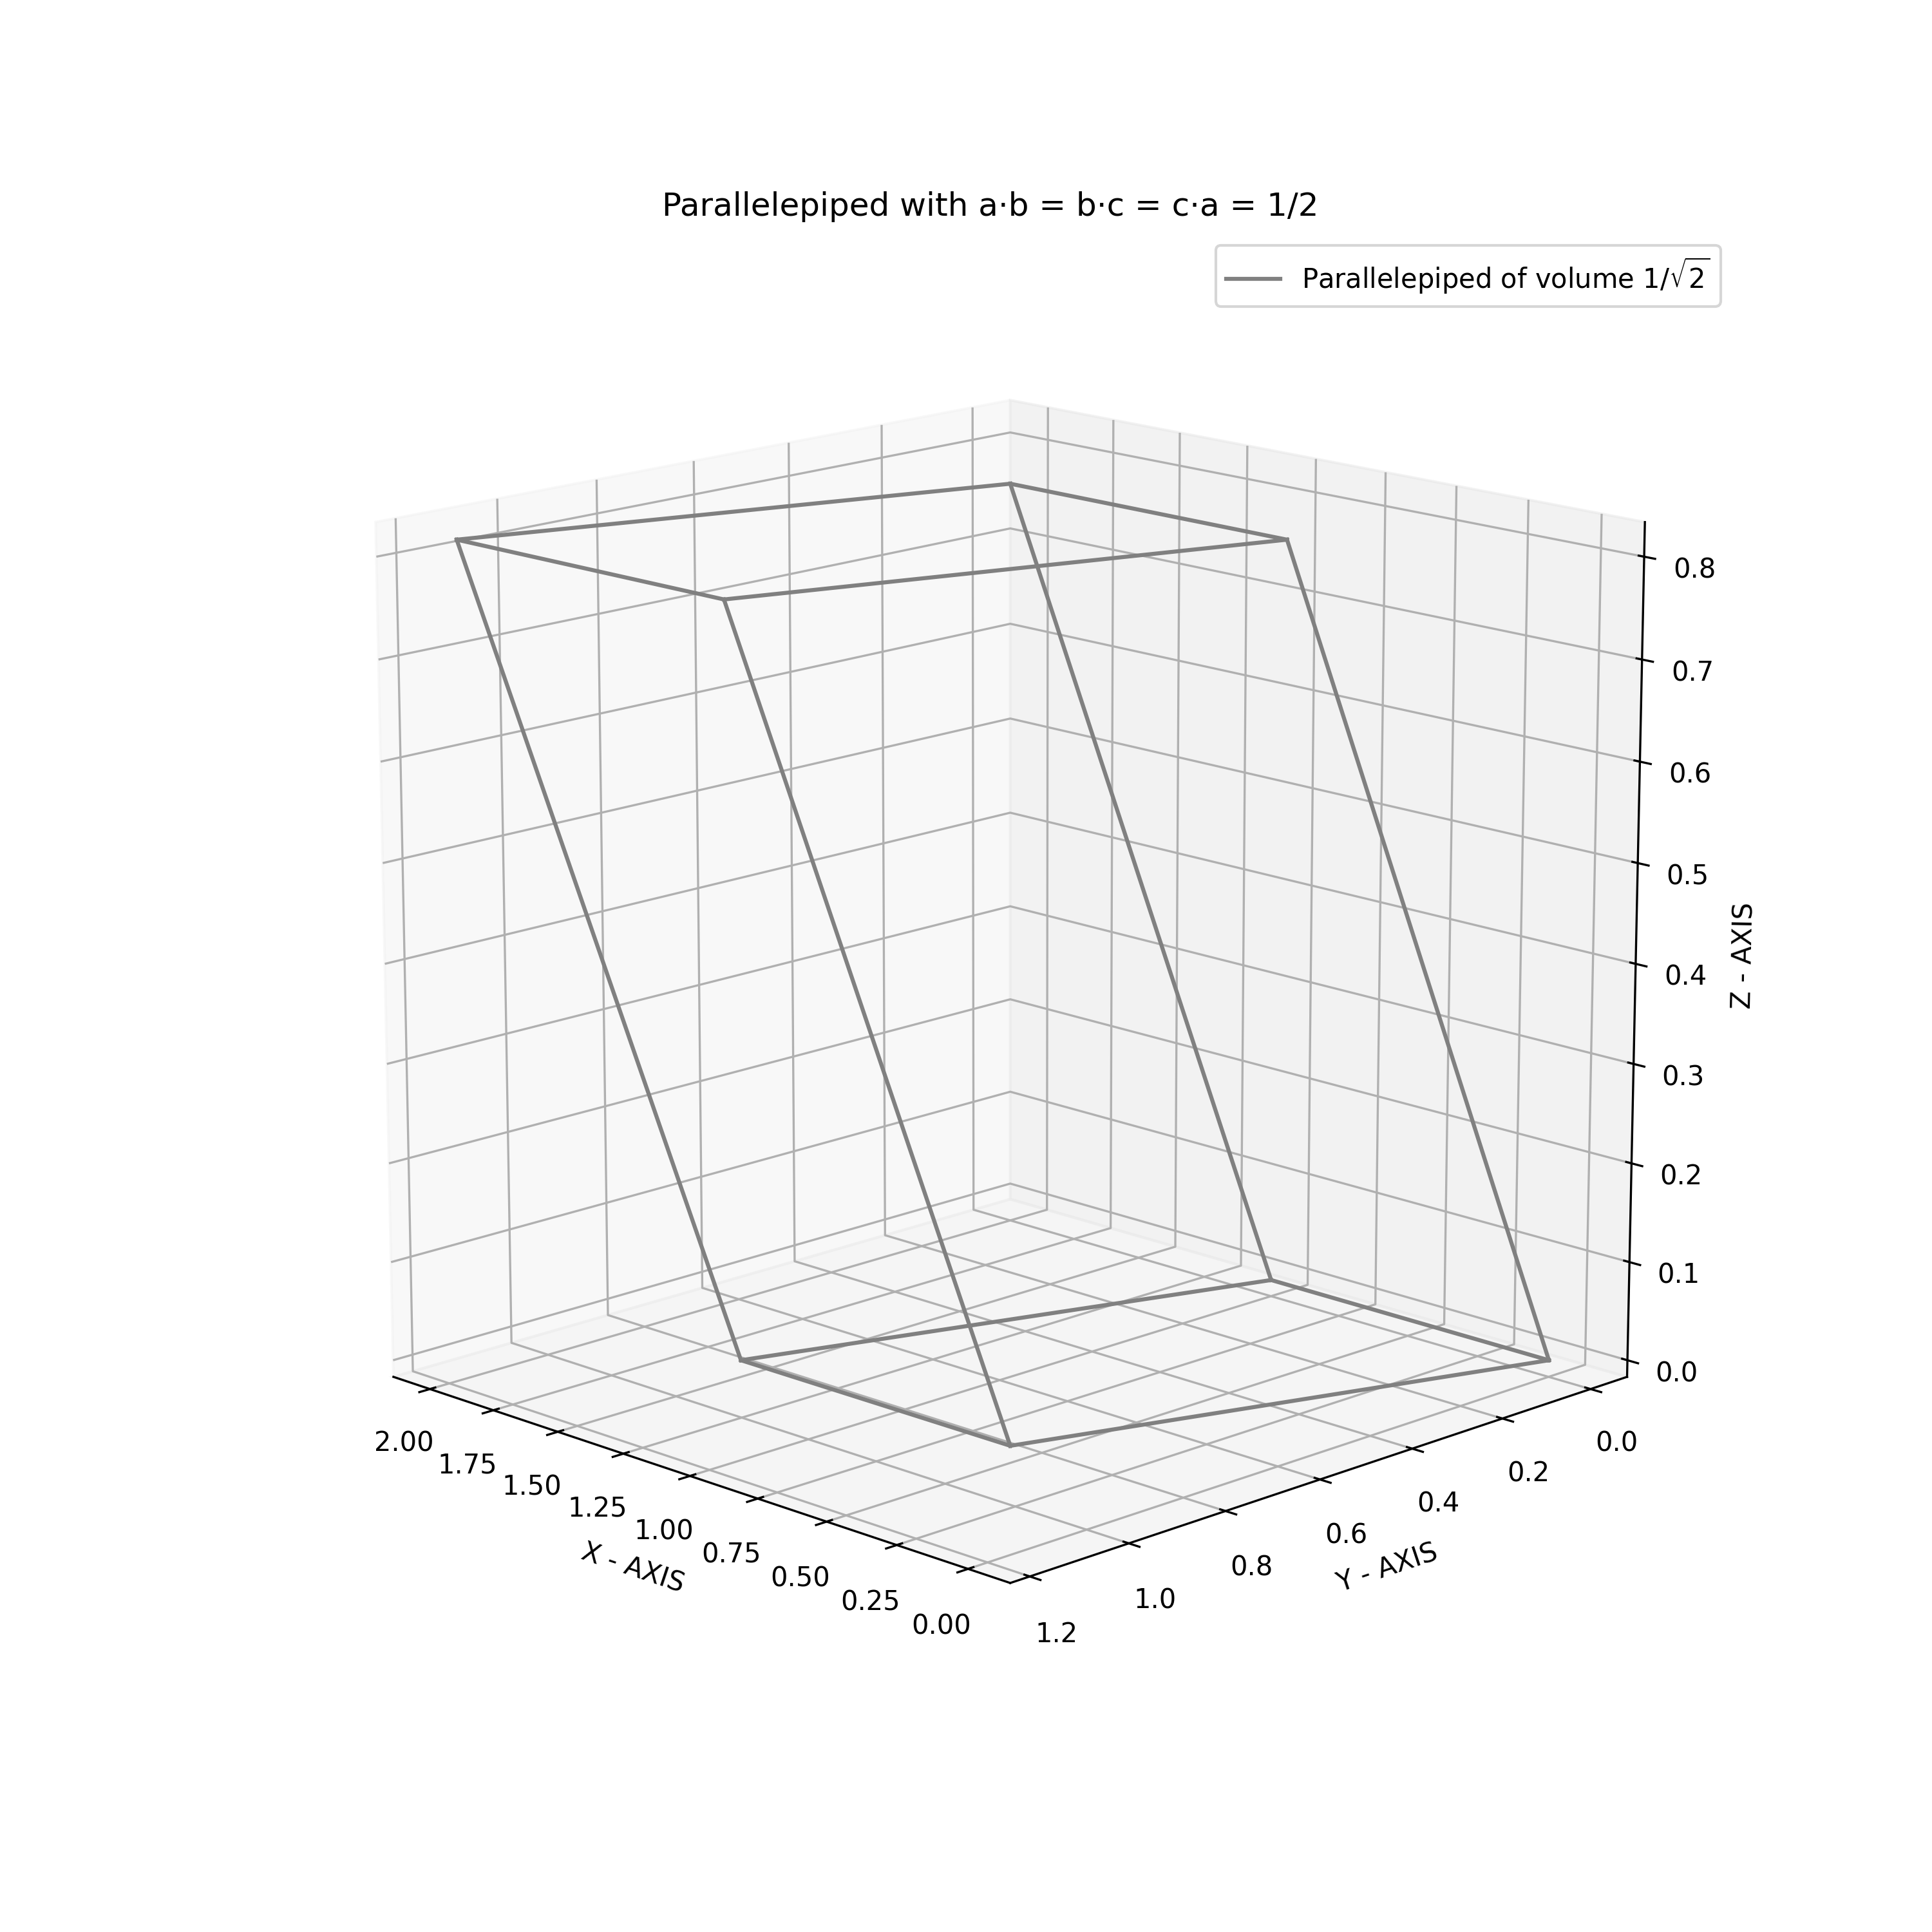
\includegraphics[width=1.0\linewidth]{figs/fig.png}
    \caption{}
    \label{fig:3DVectors}
\end{figure}

\end{document}
